The collected results give us an insight of the effect of different \textbf{ISAs} and \textbf{Cache} models on performance of code execution.

\subsection{Execution Performance}
The task done by all the ISAs in consideration is same. But the way the C code is translated to executable instruction is different in different ISAs leading different number of instructions needed to be performed to do the same amount of job. The \texttt{simInsts} parameters from results report the number of simulated instructions.


\begin{figure}[h]
	\centering
	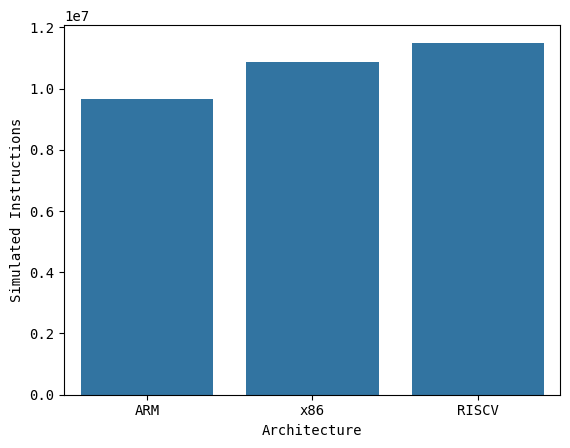
\includegraphics[width=8.5cm]{figs/inst_count.png}
	\caption{Simulated instruction count}
	\label{fig:inst_count}
\end{figure}
ARM ISA is the most efficient in terms of instruction count. The instruction count for ARM ISA is $\approx 16\%$ less than that of RISC-V ISA. The instruction count for x86 ISA is $\approx 11\%$ more than that of ARM ISA. This clearly demonstrates the efficiency of ARM ISA in terms of instruction count.
This later translates to the execution time of the code. The execution time is calculated by multiplying the instruction count with the clock cycle time. The clock cycle time is same for all the ISAs in this case. Hence, the execution time is directly proportional to the instruction count.

\begin{figure}[h]
	\centering
	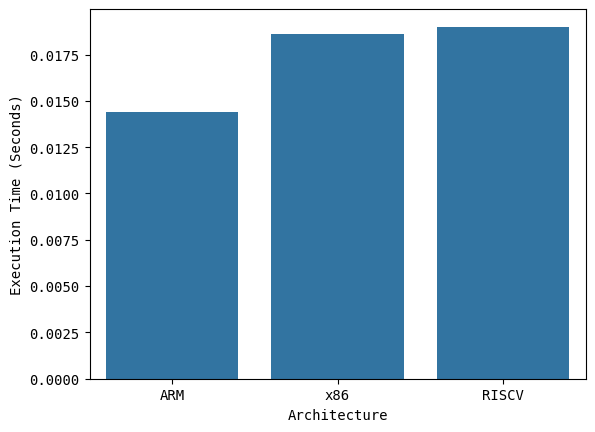
\includegraphics[width=8.5cm]{figs/exec.png}
	\caption{Execution time}
	\label{fig:exec_time}
\end{figure}

From fig~\ref{fig:exec_time}, we can see the difference in execution time as expected. But a slight deviation is observed in the execution time of x86 ISA. This deviation can be attributed to the fact that x86 ISA has higher \texttt{opcode} count than the other ISAs as seen in fig~\ref{fig:op_count} as ISAs from reduced instruction set are denser.
\begin{figure}[h]
	\centering
	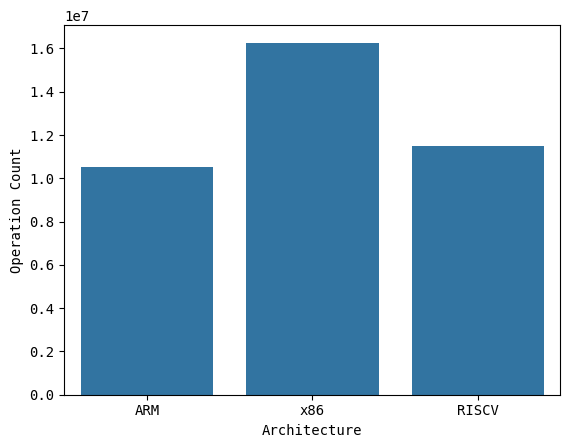
\includegraphics[width=8.5cm]{figs/op_count.png}
	\caption{Operation Count}
	\label{fig:op_count}
\end{figure}

\subsubsection{Cache Performance}

The cache performance is measured in terms of \texttt{cache\_hits} and \texttt{cache\_misses}. The cache access count represents the number of read/write operations performed on the L1 data cache, while cache misses indicate when requested data was not available in the cache and had to be fetched from main memory. The cache hit rate is calculated as:

\begin{equation}
	\mathrm{cache\_miss\_rate} = \frac{\mathrm{cache\_misses}}{\mathrm{cache\_misses} + \mathrm{cache\_hits}}
	\label{eq:cache_miss_rate}
\end{equation}

where:
\begin{itemize}
	\item $\mathrm{cache\_hits}$ is the total number of cache hits
	\item $\mathrm{cache\_misses}$ is the number of cache misses
\end{itemize}

The cache hit rate is a measure of how effectively the cache is being utilized. A higher cache hit rate indicates that the cache is able to serve a larger proportion of memory requests, leading to improved performance.
\begin{figure}[H]
	\centering
	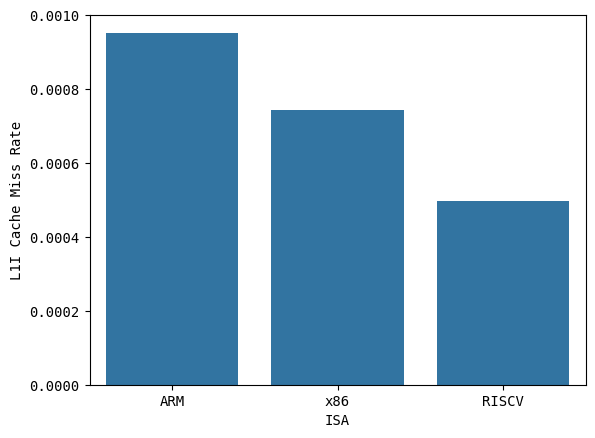
\includegraphics[width=8.5cm]{figs/l1i.png}
	\label{fig:l1i_cache}
\end{figure}
\begin{figure}[H]
	\centering
	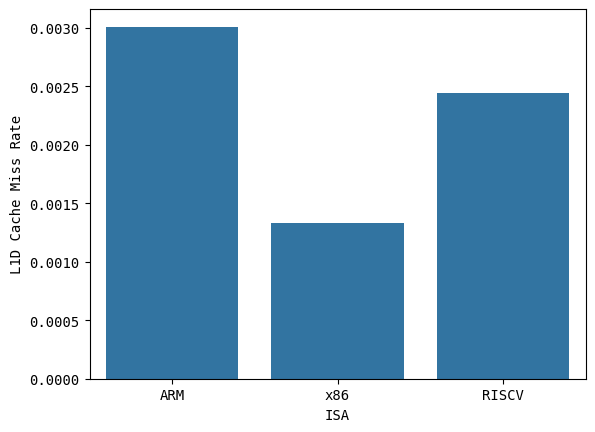
\includegraphics[width=8.5cm]{figs/l1d.png}
	\label{fig:lid_cache}
\end{figure}
\begin{figure}[H]
	\centering
	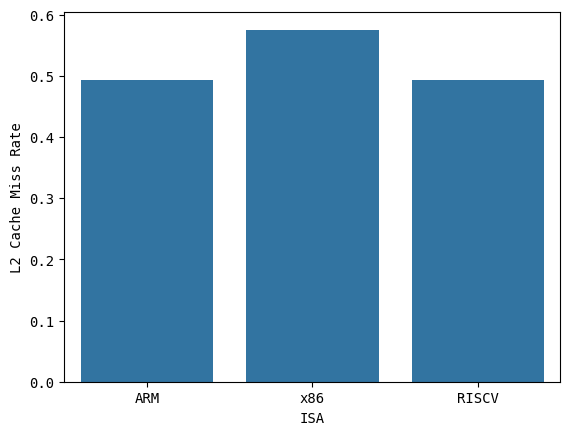
\includegraphics[width=8.5cm]{figs/l2.png}
	\caption{Cache performance}
	\label{fig:l2_cache}
\end{figure}

The \texttt{L1I} cache miss rate is the lowest among all the ISAs. This indicates that the instruction cache is able to serve a larger proportion of memory requests, leading to improved performance. This is expected as the instruction cache is designed to store frequently accessed instructions, which are likely to be reused. The \texttt{L1D} cache miss rate is also low, indicating that the data cache is able to serve a large proportion of memory requests. The \texttt{L2} cache miss rate is higher than the \texttt{L1D} cache miss rate, indicating that the L2 cache is not able to serve as many memory requests as the L1 cache. This is expected as the \texttt{L2} cache is designed to store less frequently accessed data.

\begin{table}[H]
	\centering
    \caption{Cache Performance Classification}
	\begin{tabular}{ll}
		\toprule
		Hit Rate Range & Interpretation                      \\
		\midrule
		$>90\%$        & Excellent temporal/spatial locality \\
		$60-90\%$      & Partial working set fit             \\
		$<60\%$        & Poor cache utilization              \\
		\bottomrule
	\end{tabular}
	\label{tab:cache_class}
\end{table}

The RISC family of ISAs have the best cache performance.

\begin{figure}[H]
	\centering
	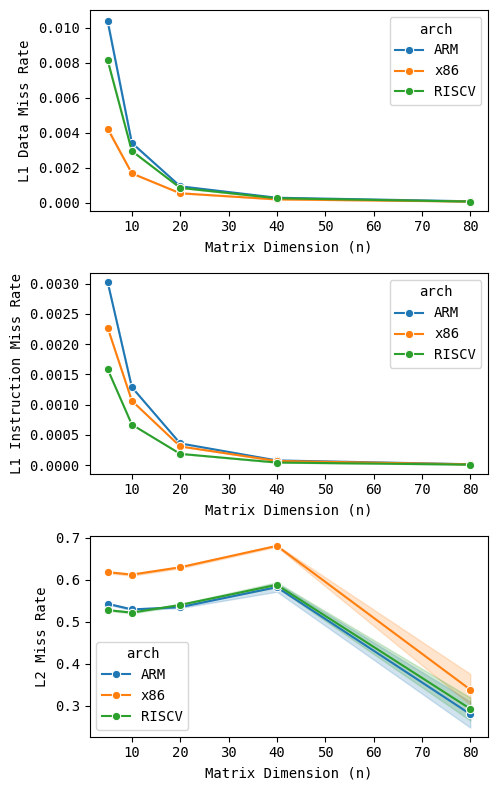
\includegraphics[width=8.5cm]{figs/dim_cache.png}
    \caption{Cache performance vs matrix size}
	\label{fig:dim_cache}
\end{figure}
Fig \ref{fig:dim_cache} shows the cache performance vs matrix size. The cache hit rate increases with increase in matrix size. This is expected as the larger the matrix size, the more data is likely to be reused, leading to better cache performance.